\documentclass[11pt]{article}
\usepackage{float}
\usepackage{graphicx}
\usepackage{lscape}
\usepackage{pdflscape}
\usepackage{booktabs}
\usepackage{natbib}
\usepackage{pdfpages}
\usepackage[acronym, toc, nonumberlist]{glossaries}
\usepackage{url} 
\usepackage{hyperref}
\usepackage{xcolor}
\hypersetup{
    colorlinks,
    linkcolor={red!50!black},
    citecolor={blue!50!black},
    urlcolor={blue!80!black}
}
% \usepackage[none]{hyphenat}

\newcommand{\figref}[1]{\hyperref[#1]{\figurename~\ref*{#1}}}


\makeglossaries
\newacronym{iot}{IoT}{Internet of Things}
\newacronym{coap}{CoAP}{The Constrained Application Protocol}
\newacronym{udp}{UDP}{User Datagram Protocol}
\newacronym{rest}{REST}{Representational State Transfer}
\newacronym{m2m}{M2M}{Machine-to-Machine}
\newacronym{rpi}{RPi}{Raspberry Pi}
\newacronym{json}{JSON}{JavaScript Object Notation}
\newacronym{gpio}{GPIO}{General Purpose Input Output}

\title{CoAP based IoT data transfer from a Raspberry Pi to Cloud}
\author{Thomas Scott}
\date{20th November 2018}

\begin{document}
	\pagenumbering{gobble}
	\maketitle
	\newpage
	\pagenumbering{arabic}

	\section{Abstract}
	This research investigates the use of \gls{coap} in transmitting sensor data
to the cloud. It aims to explore how \gls{coap} fits into the \gls{iot} ecosystem and
what advantages, if any, it offers over other \gls{iot} protocols. A framework is proposed 
using a \gls{rpi} and sensor acting as an \gls{iot} endpoint. This endpoint will allow for
\gls{coap} requests and will poll the sensor and return the latest data as \gls{json}.
The endpoint will be polled from a cloud service, this service will then display the data to 
the user.

	\section{Introduction}
	The reduced cost of low powered small devices, such as the \gls{rpi}, has made it more accessible to create bespoke systems. 
This combined with the increasing popularity of home automation allows for these devices to be used in the \gls{iot}.

The \gls{iot} can be viewed as a large distributed network comprising of highly dynamic devices \citep{miorandi2012internet}. Small low powered ``smart'' devices can connect and communicate with one another. Some of these devices can contain or communicate with sensors that record real world data. This data can then be transmitted to other devices allowing them to trigger actions. In this way groups of smart devices can be used to improve day to day situations such as automated houses (thermostats and heating etc.), security and improved monitoring.

The Raspberry Pi \citep{pi3model} is a credit card sized computer developed by the Raspberry Pi Foundation. 
The \gls{rpi}'s ability to act as a GNU/Linux server and the interfacing services provided by its general purpose I/O pins make it a popular 
choice of hardware for \gls{iot} applications. \citep{kumar2016iot}

With 48\% of the UK market considering their smartphone as the most important device for internet access \citep{ofcom2018} allowing users to use their handheld devices to view and manage their data has become increasingly necessary. Cloud platforms that allow access from any device go a long way to 
solving this problem. Storing sensor data in the cloud allows for easy access to users from any device as well as allowing for scalable storage.

As these devices are limited in computing power it is important that the devices communicate efficiently. 
This paper explores the use of \gls{coap} as a protocol to transmit sensor data from a small, low powered device (\gls{rpi}) to send sensor data to the cloud.

In this system the a sensor will be attached to the \gls{rpi}, the \gls{rpi} will be responsible for taking the data from the sensor and then 
using the \gls{coap} protocol to transmit this data to the cloud platform.

	\section{Design}
	The system shall consist of four main elements: the sensor, the \gls{rpi}, \gls{coap} and the cloud platform.
The sensor will collect the data and pass this to the \gls{rpi}. The \gls{rpi} will then be responsible for manipulating
the data into a suitable format for transmission via \gls{coap}. The implementation of \gls{coap} will communicate with
the cloud platform. The cloud platform will store the data, allowing access to users.

\begin{figure}[H]
    \centering
    \makebox[1\textwidth]{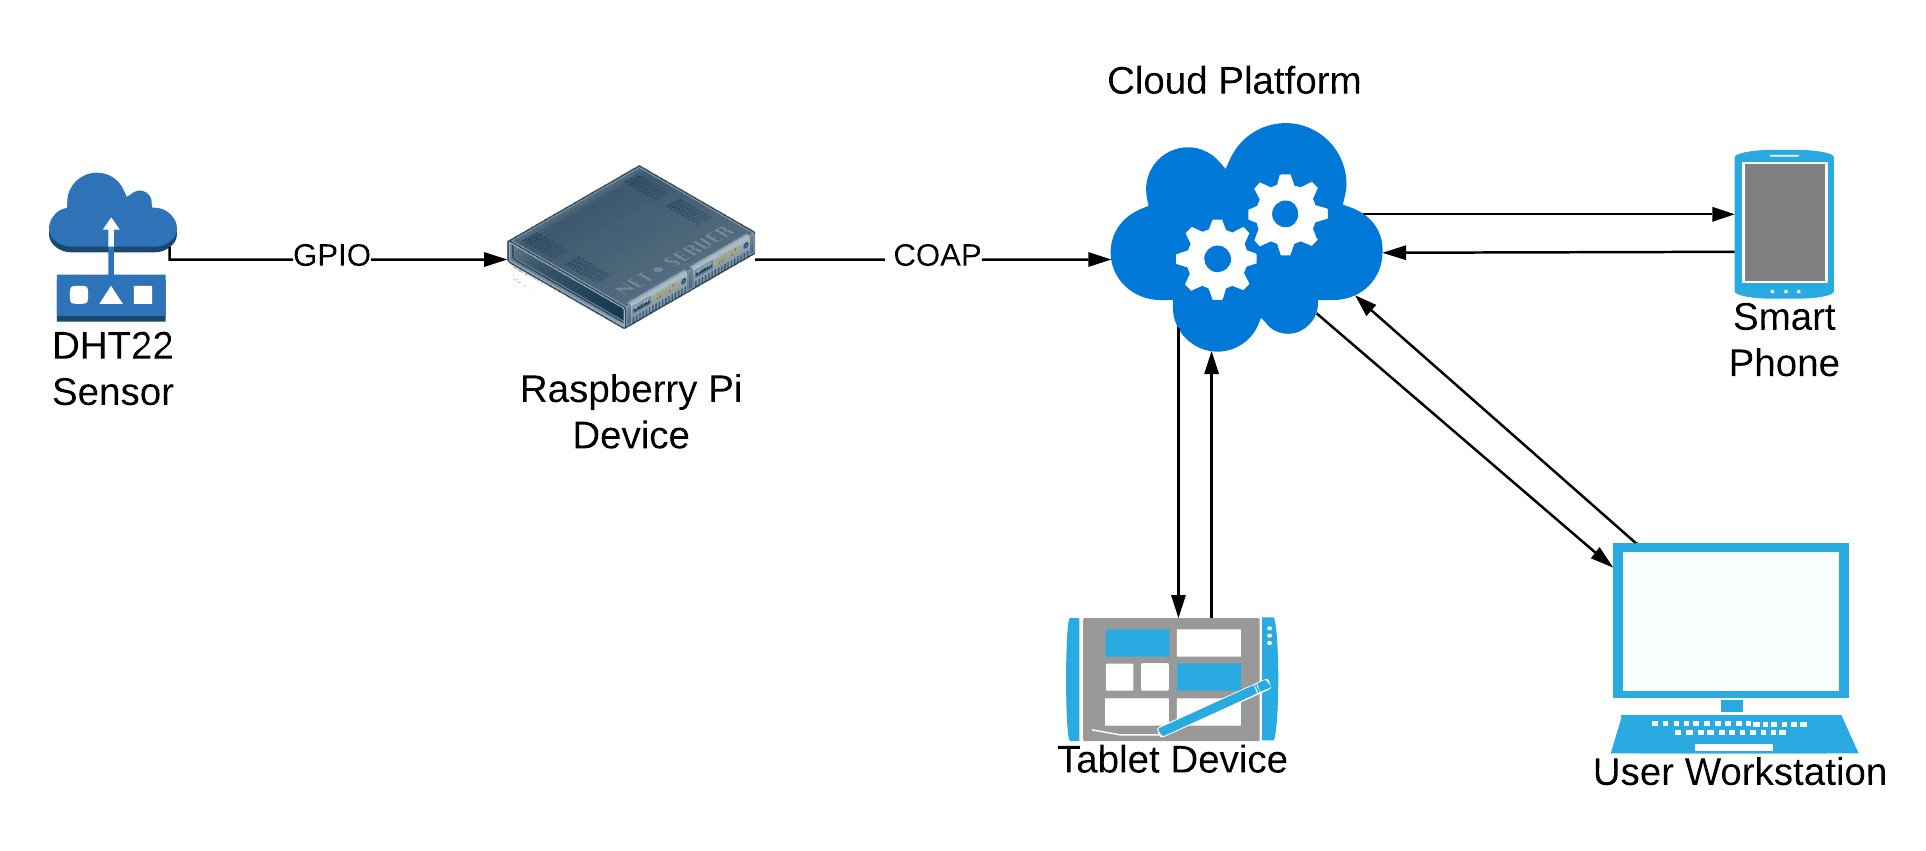
\includegraphics[width=1\textwidth]{assets/Project_Framework.png}}
    \caption{\label{fig:proj_framework} The project infrastructure.}
\end{figure}

The DHT22 sensor will connect to the \gls{rpi} using the \gls{rpi}'s on board \gls{gpio} ports as shown in \figref{fig:rpi_wiring}. 
A Python script using the AdaFruit Python DHT package to retrieve data from the sensor and the CoAPthon Python library will format the sensor data as 
\gls{json}. This script will then make the \gls{json} data available as a \gls{coap} endpoint from which the cloud service can get or subscribe to 
the latest data. 


\begin{figure}[H]
    \centering
    \makebox[1\textwidth]{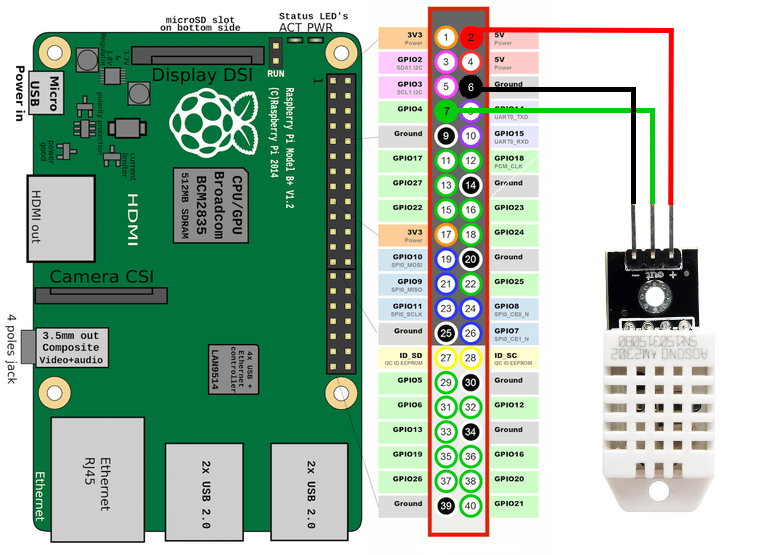
\includegraphics[width=1\textwidth]{assets/rpi_wiring.png}}
    \caption{\label{fig:rpi_wiring} Wiring diagram for connecting the sensor to the \gls{rpi}.}
\end{figure}

\begin{figure}[H]
    \centering
    \makebox[1\textwidth]{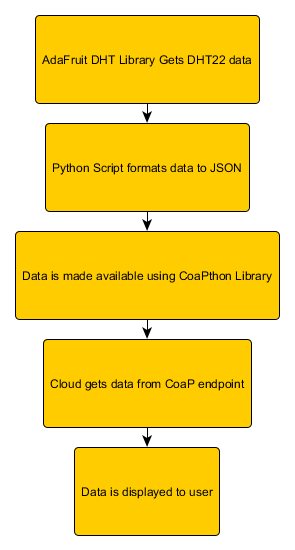
\includegraphics[width=0.5\textwidth]{assets/data_flow.png}}
    \caption{\label{fig:data_flow} Shows the flow of data from sensor to user.}
\end{figure}


	\section{Methodology}
	The aim of the proposed system is to investigate the implementation of \gls{coap} on a \gls{rpi} and how \gls{coap} can be 
used to transmit data to the cloud. 

To achieve this a \gls{coap} endpoint will need to be created on the \gls{rpi}. The \gls{rpi} will collect sensor data at intervals and store them 
locally on the device. The \gls{rpi} will act as a \gls{coap} server that will respond to \gls{rest} GET requests with the sensor data and the time
the reading was taken in a \gls{json} format.

The clouds responsibility will be to send the GET requests to the \gls{coap} endpoint hosted on the \gls{rpi} and to receive and store the data
returned. The cloud should send a confirmable request to the \gls{coap} endpoint. The \gls{coap} endpoint should then respond with an acknowledgement. 
If the data is available, the data should be ``piggybacked'' to this response, as shown in Figure \figref{fig:coap_get_piggy}, if not the data should be 
returned in a confirmable message containing the data.
 In this case the cloud client will then send it's own acknowledgement message to the \gls{coap} endpoint. This is shown in  \figref{fig:coap_get_delayed}.

\begin{figure}[H]
    \centering
    \makebox[1\textwidth]{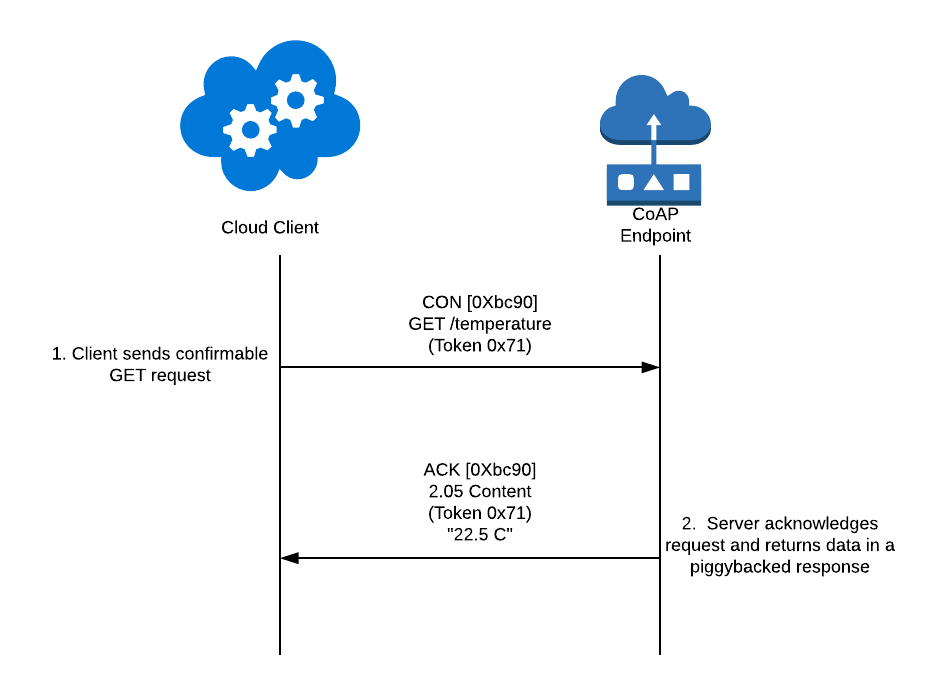
\includegraphics[width=1\textwidth]{assets/coap_get_request.png}}
    \caption{\label{fig:coap_get_piggy} Example \gls{coap} GET request with piggybacked response. \citep{bormann2015constrained}}
\end{figure}

With \gls{coap} endpoints acting as both a client, that sends requests, and a server implementation of \gls{coap} will be needed 
in each the \gls{rpi} and the cloud platform. The \gls{rpi} will then regularly retrieve readings from the sensor and send a POST request 
at intervals to the cloud \gls{coap} endpoint. This approach will be contrasted with the cloud server observing the \gls{rest} endpoint on the \gls{rpi}.
The results of both approaches will be evaluated.

\begin{figure}[H]
    \centering
    \makebox[1\textwidth]{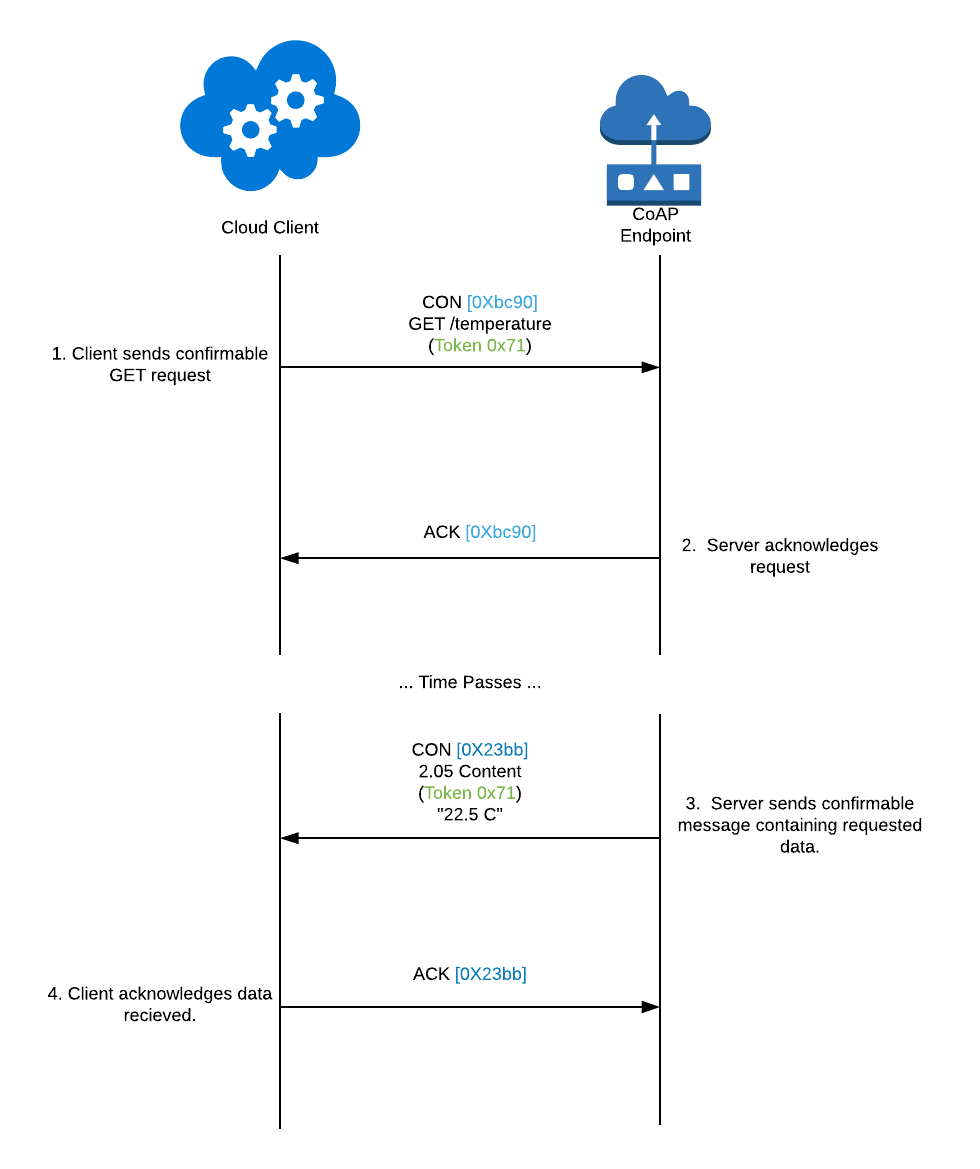
\includegraphics[width=1\textwidth]{assets/coap_get_delayed.png}}
    \caption{\label{fig:coap_get_delayed} Example \gls{coap} GET request without piggybacked response. \citep{bormann2015constrained}}
\end{figure}


	\section{Software and Hardware specification}
	\subsection{Hardware}
\begin{enumerate}
    \item Raspberry Pi 3

        Raspberry Pi 3 Model B, includes built in WiFi, \gls{gpio} ports and a 1.2GHz Quad-Core processor.
    \item Micro SD card
    
        Used to load operating system onto the \gls{rpi}.
    \item Power cord
    
        Supplies power to the \gls{rpi}.
    \item DHT22 temperature and humidity sensor
    
        Connects to the \gls{rpi} using the \gls{rpi}'s \gls{gpio} ports. Will be used to provide data.

\end{enumerate}

\subsection{Software}
\begin{enumerate}
    \item Python 3

        The Python programming language will be used to create the scripts and software needed on the \gls{rpi}.
        This is due to the languages popularity when creating projects on the \gls{rpi} and the languages wide selection
        of networking packages.
    \item CoAPthon
    
        Python implementation of \gls{coap}. Licensed under the MIT license. \href{https://github.com/Tanganelli/CoAPthon}{Github}.

    \item AdaFruit Python DHT
        
        Python library to retrieve sensor data from the DHT22. \href{https://github.com/adafruit/Adafruit_Python_DHT}{Github}.

    \item Git Version Control
    
        Source code version control system to allow for adjustments to the code.

    \item Cloud Platform
    
        Will act as an end point to the \gls{rpi} where the sensor data will be stored.
\end{enumerate}

	\section{Conclusion}
	This research investigates the use of \gls{coap} in transmitting sensor data
to the cloud. It aims to explore how \gls{coap} fits into the \gls{iot} ecosystem and
what advantages, if any, it offers to other protocols. It also shows how a \gls{rpi} can
be used with Python to create an \gls{iot} device and connect to the cloud. 

	\printglossaries

	\bibliographystyle{agsm}
	\bibliography{references}
\end{document}

